% !TEX program = xelatex

\documentclass[10pt, compress,notheorems]{beamer}

\usetheme{m}

\usepackage{booktabs}
\usepackage[scale=2]{ccicons}
\usepackage{minted}
\usepackage{amsmath}
\usepackage{bm}
\usepackage{hyperref}
\usepackage{url}
\usepackage{graphicx}
\usepackage{multirow}
\usepackage{multicol}
\usepackage{amsfonts}
\usepackage{pgf,tikz}
\usepackage{tgpagella}
\usepackage{centernot}
\usepackage{caption}
\usepackage{xcolor}

\usepackage{graphicx}

\usepackage{xspace}
\newcommand{\themename}{\textbf{\textsc{metropolis}}\xspace}

\usepgfplotslibrary{dateplot}

\usemintedstyle{trac}

\title[Text Analysis]{Text Analysis}
\subtitle{}
\date{}
\author{
    \href{mailto:christopher.gandrud@city.ac.uk}{Christopher Gandrud}
}
\institute{SG1022, City University London}

\begin{document}

\maketitle

\frame{
    \frametitle{Aims}

    \begin{itemize}

        \item What is text analysis and why use it?

        \item Human vs. machine coding

        \item The general process

        \item Specific issues with machine coding

        \item Pros and Cons

    \end{itemize}

}

\section{Defining text analysis}

\frame{

    \begin{center}
        ``When we perform textual analysis on a text, we make an {\large{educated guess}} at some of the {\large{most likely interpretations}} that might be made of that text.'' {\small{(McKee 2003, 1)}}
    \end{center}
}

\frame{
    \frametitle{Define content analysis}

    \begin{center}
        ``{\large{Content Analysis}} is a research technique for making {\large{replicable and valid inferences}} from texts (or other meaningful matter [e.g. videos, audio]) to the {\large{contexts}} of their use.'' {\small{(Krippendorff 2013, 24)}}
    \end{center}
}

\frame{
    \frametitle{Replicable}

    \begin{center}
        \textcolor{gray}{``Content Analysis is a research technique for making {\large{replicable}} and valid inferences from texts (or other meaningful matter [e.g. videos, audio]) to the contexts of their use.''}
    \end{center}

    {\large{Replicable}}: different researchers, independent of each other should get the same results when applying the same technique.

    \vspace{0.5cm}

    Replicable results are more reliable.

}

\frame{
    \frametitle{Valid}

    \begin{center}
        \textcolor{gray}{``Content Analysis is a research technique for making replicable and {\large{valid}} inferences from texts (or other meaningful matter [e.g. videos, audio]) to the contexts of their use.''}
    \end{center}

    {\large{Valid}}: research is open to careful scrutiny and your claims can be upheld given independently available evidence.
}

\frame{
    \frametitle{Texts}

    \begin{center}
        \textcolor{gray}{``Content Analysis is a research technique for making replicable and valid inferences from {\large{texts}} (or other meaningful matter [e.g. videos, audio]) to the contexts of their use.''}
    \end{center}

    {\large{Texts}}: something that is produced by someone to have meaning for someone else.

    \vspace{0.5cm}

    E.g. newspaper articles, treaties, transcripts, tweets, maps, advertisements, press releases, movies, party manifestos.

    \vspace{0.5cm}

    In this course we focus exclusively on written texts composed of words.

}

\frame{
    \frametitle{Texts in contexts}

    \begin{enumerate}

        \item<1-> Texts have no objective--reader-independent qualities. Meaning (data) arises from someone reading the text, often expecting other's understanding.

        \item<2-> Texts do not have single meanings.

        \item<3-> Meanings invoked by texts need not be shared.

        \item<4-> Contents refer to something other than themselves.

        \item<5-> Texts have meanings relative to particular contexts.

        \item<6-> Content analysts infer answers to particular research questions from their texts. Their inferences are merely more systematic, explicitly informed, and verifiable \ldots than what ordinary readers do.
    \end{enumerate}

}

\section{Why use text analysis?}

\frame{
    \frametitle{You}

    \begin{center}
        {\large{You \emph{use} and \emph{contribute} to text analysis}} {\large{every day.}}
    \end{center}
}

\frame{

    \begin{center}
        
\includegraphics[scale=0.45]{img/google_search_kanye.png}
    \end{center}
}

\frame{

    \begin{center}
        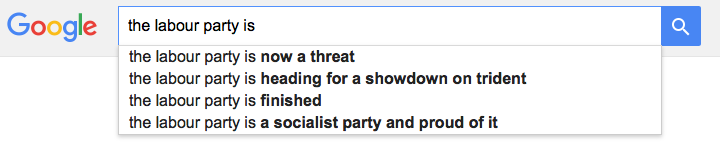
\includegraphics[scale=0.45]{img/google_search_labour.png}
    \end{center}

}

\frame{
    \frametitle{You}

    \begin{center}
        {\large{(Some of you) are building a data set that will be used for text analysis}} {\LARGE{right now}}.
    \end{center}

}

%\frame{

%    \begin{center}
%        
\includegraphics[scale=0.45]{img/whats_app.png}
%    \end{center}

%    {\tiny{Source: http://www.buzzfeed.com/shayanroy/blocking-you-now#.obE7eXDgAP}}

%}

\frame{

    \begin{center}
        
\includegraphics[scale=0.4]{img/facebook.png}
    \end{center}

{\tiny{Source: http://www.buzzfeed.com/jessicamisener/stupidest-things-ever-said-on-facebook#.elRz03arDM}}

}

\frame{
    \frametitle{Social Science}

    \begin{center}
        People are creating {\large{increasingly more}} (machine accessible) texts.

        \vspace{1cm}

        {\large{Massive new source of data}} for social science analysis.
    \end{center}

}

\frame{
    \frametitle{Text analysis in social science (examples)}

    We may have research questions where we conducted a survey with an {\large{open-ended question}}.

    \vspace{1cm}

    We need some {\large{systematic way}} to {\large{understand}} these texts and {\large{make comparisons}} across survey respondents.

}

\frame{
    \frametitle{Text analysis in social science (examples)}

    We may have research questions where we want to interview a group of people that are hard to access, but who produce many texts.

    \vspace{1cm}

    For example, in an ideal world we may want to survey world leaders for their preferences for handling Syrian refugees. We may want to see how these preferences change over time.

    \vspace{1cm}

    World leaders don't given many interviews (especially not multiple interviews on the same topic), but they--often filtered through a press office--do create many texts.

}

\frame{
    \frametitle{German Chancellory Press Release Sept. 2015}


    \begin{center}
        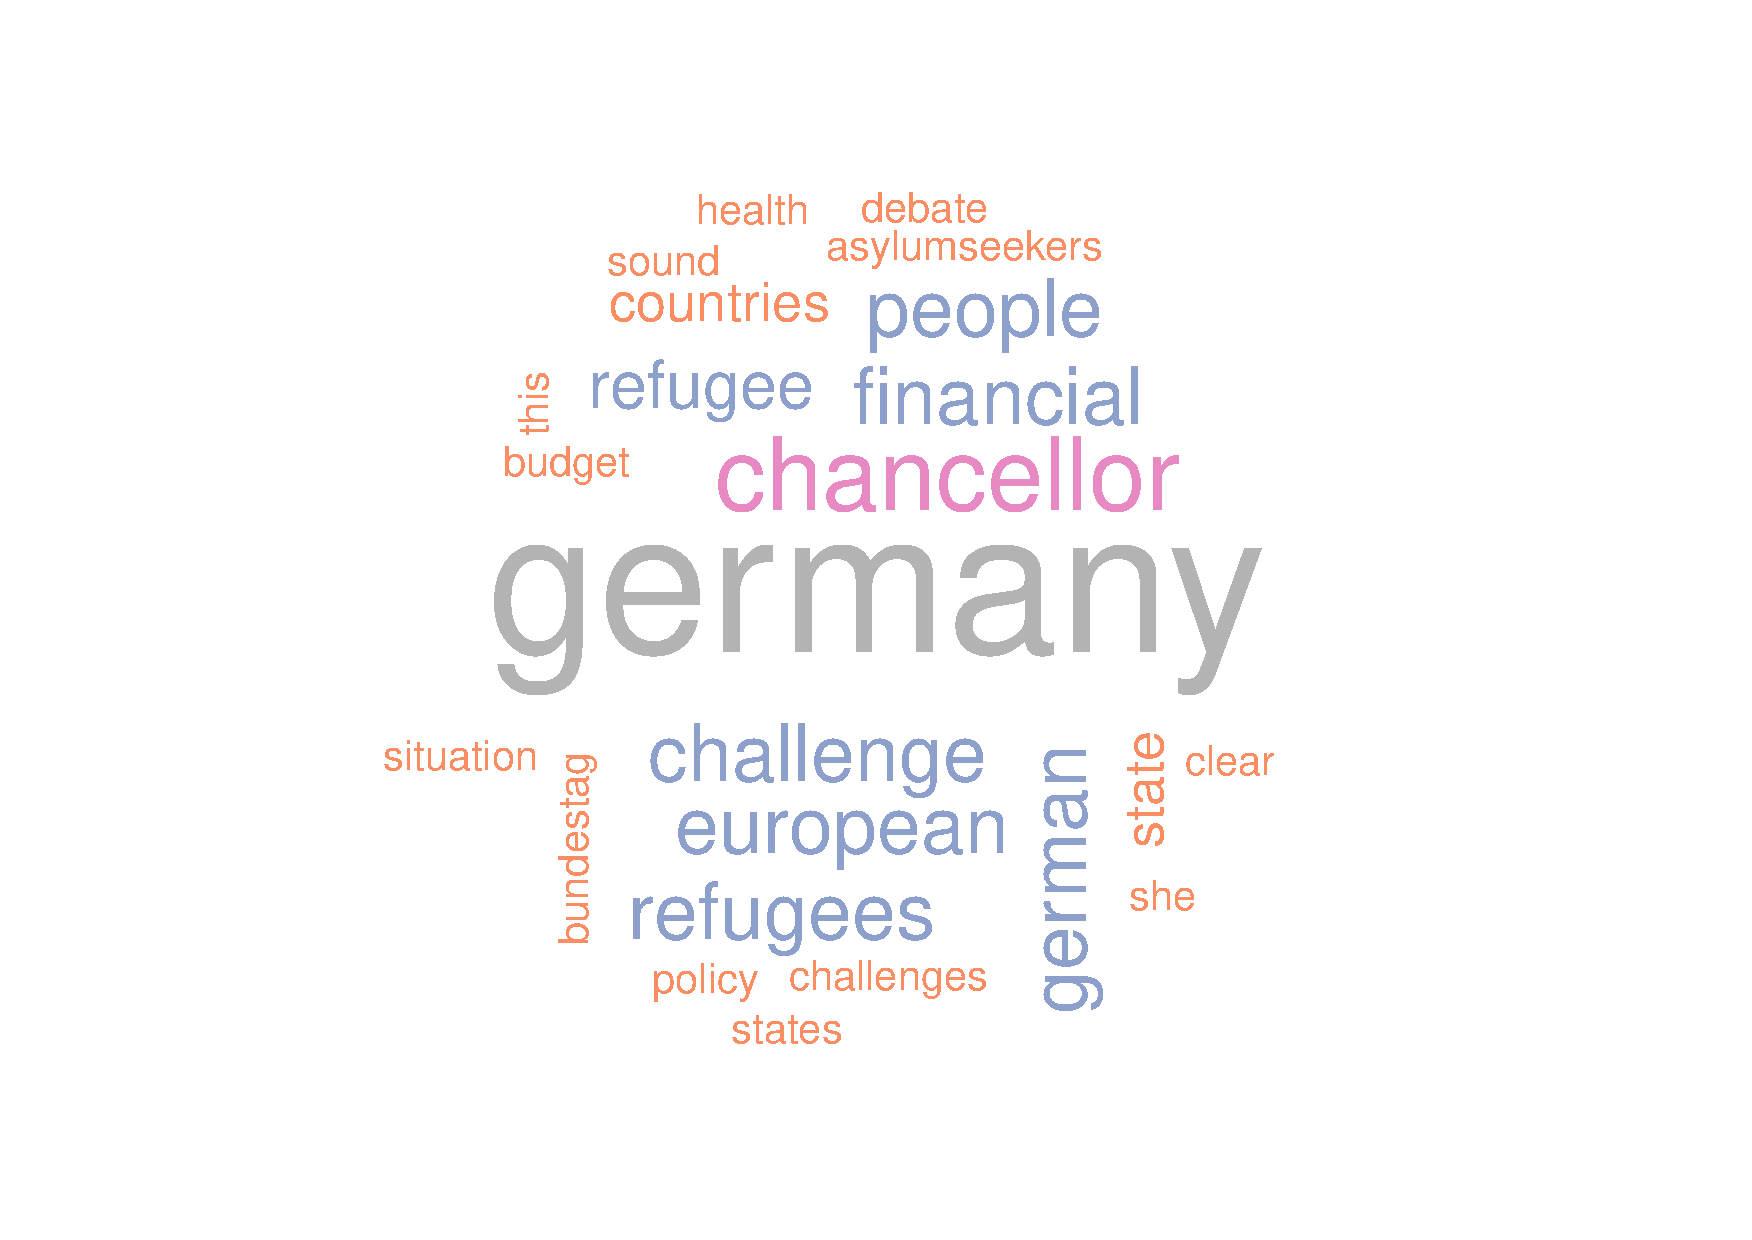
\includegraphics[scale=0.35]{img/sept_chancellor.pdf}
    \end{center}

}

\frame{
    \frametitle{Cologne New Years Eve Assults}

    \begin{center}
        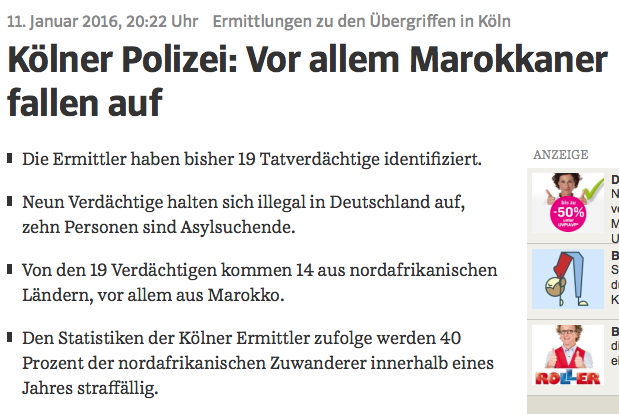
\includegraphics[scale=0.35]{img/sd_deutsche.png}
    \end{center}

    {\tiny{Source: http://www.sueddeutsche.de/panorama/ermittlungen-zu-den-uebergriffen-in-koeln-vor-allem-marokkaner-fallen-auf-1.2814336}}

}

\frame{
    \frametitle{Cologne New Years Eve Assults}

    \begin{center}
        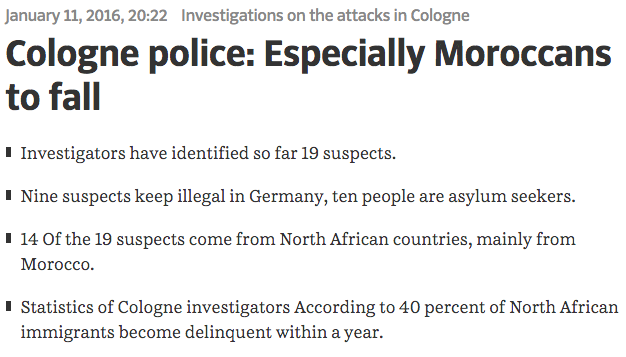
\includegraphics[scale=0.35]{img/sd_english.png}
    \end{center}

    {\tiny{Source: http://www.sueddeutsche.de/panorama/ermittlungen-zu-den-uebergriffen-in-koeln-vor-allem-marokkaner-fallen-auf-1.2814336 via Google Translate}}

}

\frame{
    \frametitle{German Chancellory Press Release January 2015}


    \begin{center}
        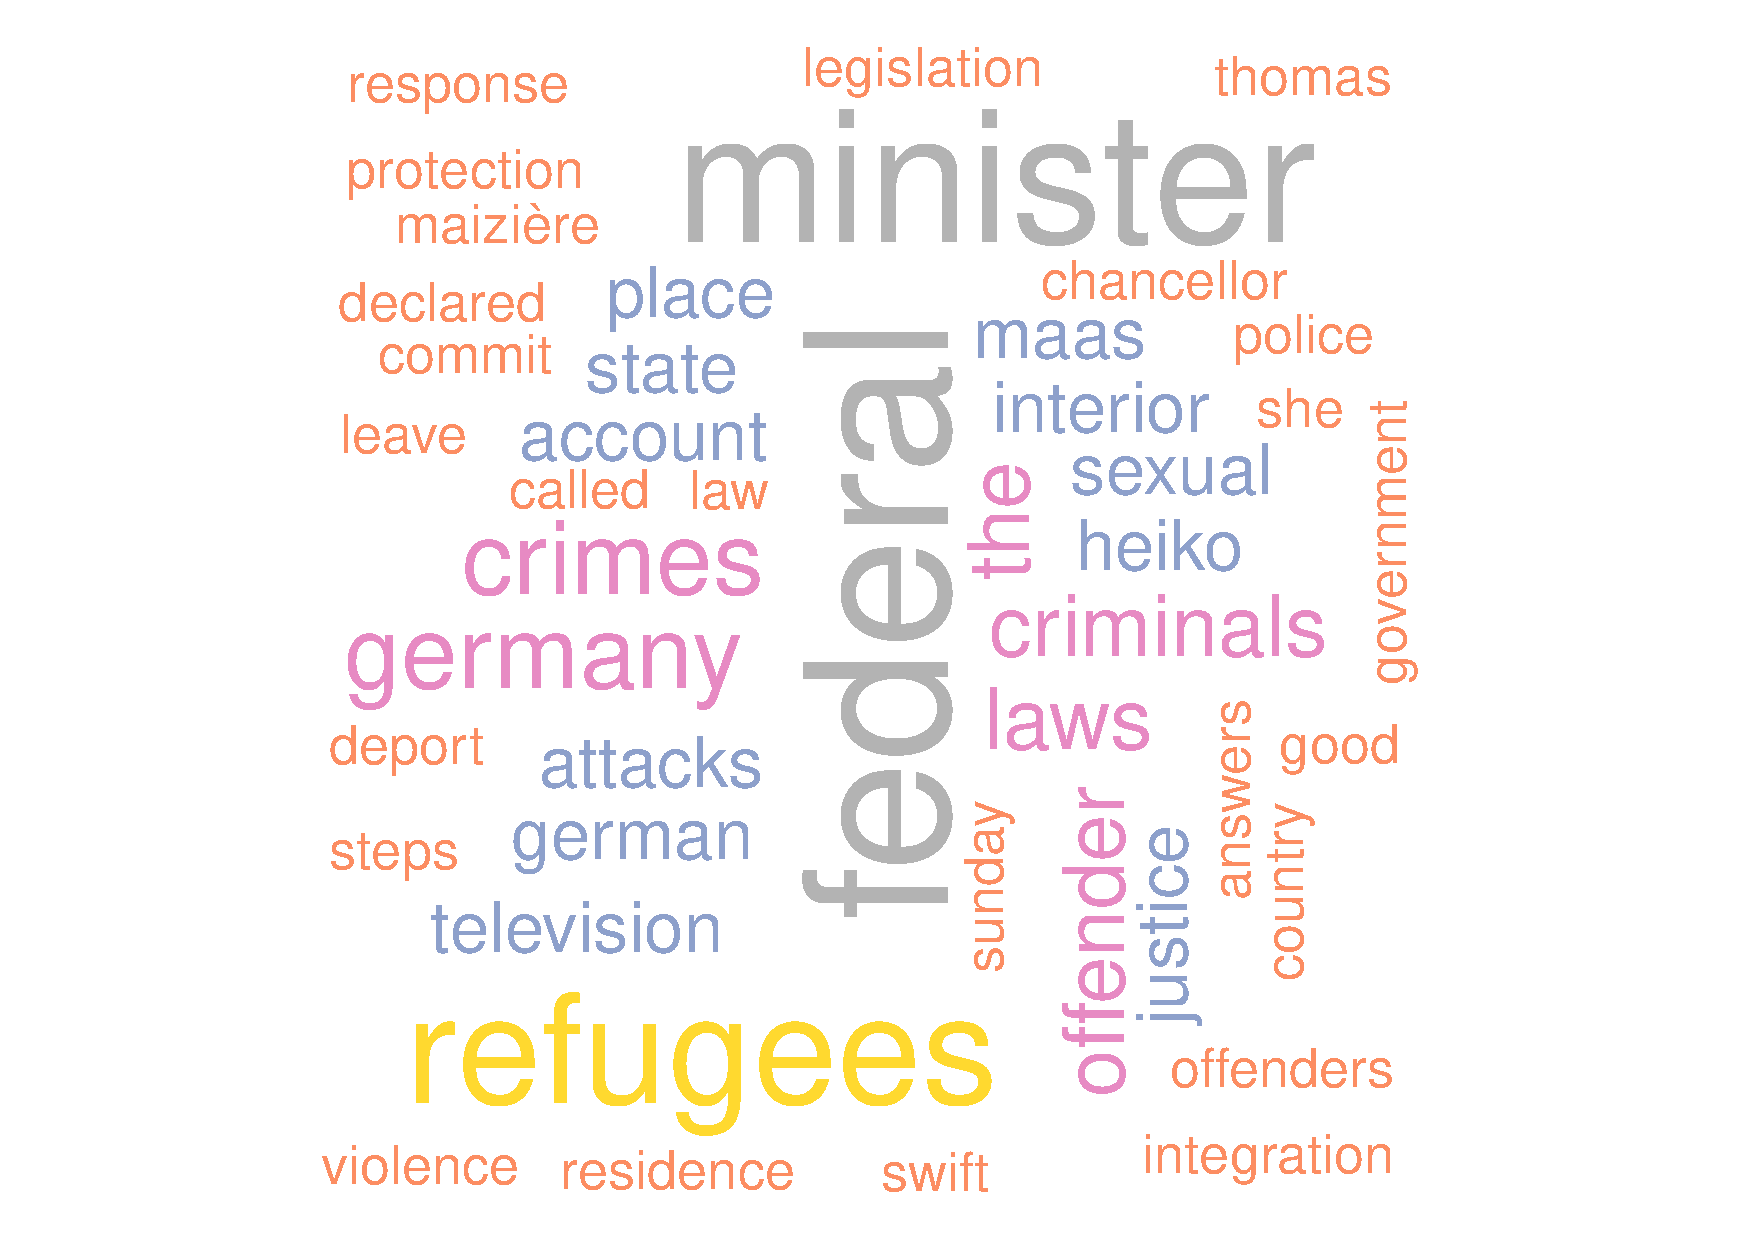
\includegraphics[scale=0.35]{img/jan_chancellor.pdf}
    \end{center}

}

\frame{
    \frametitle{Text analysis in social science (examples)}

    We may have research questions about units that are not able to answer a questionnaire, but which produce texts.

    \vspace{1cm}

    E.g. International organisations, political parties, neighbourhood groups.
}

\frame{
    \frametitle{Comparative Party Manifestos Project}

    Left-Right Position of UK Parties Based on their Party Manifestos

    \begin{center}
        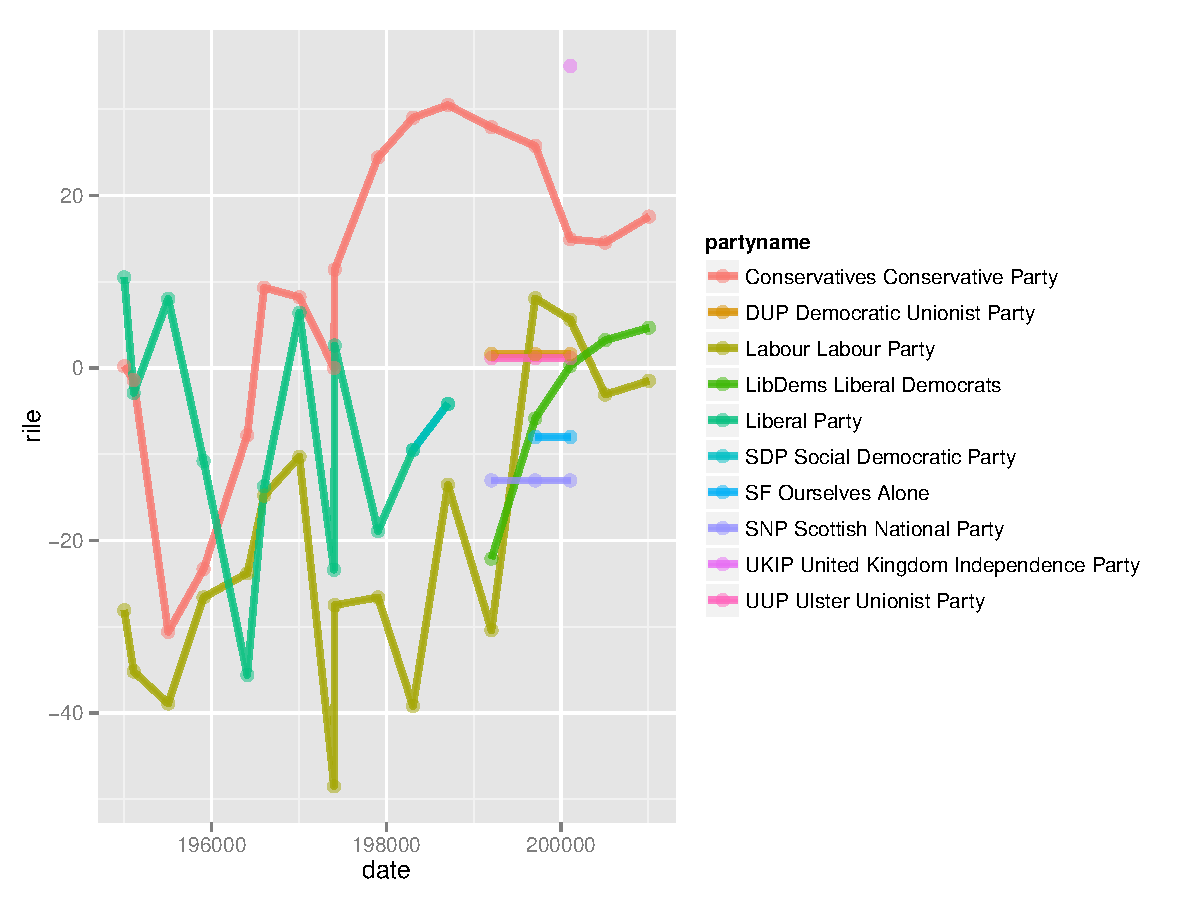
\includegraphics[scale=0.4]{img/uk_party_lr.pdf}
    \end{center}

    {\tiny{Source: https://visuals.manifesto-project.wzb.eu/mpdb-shiny/cmp\_dashboard/}}

}

\frame{
    \frametitle{Text analysis in social science (examples)}

    We may have research questions about {\large{how actors communicate}} to achieve goals.

    \vspace{1cm}

    For example, what topics do monetary policy bureaucrats talk about more when there is a financial crisis?

}

\frame{
    \frametitle{Topics of US Federal Reserve Governor Speeches}


    \begin{center}
        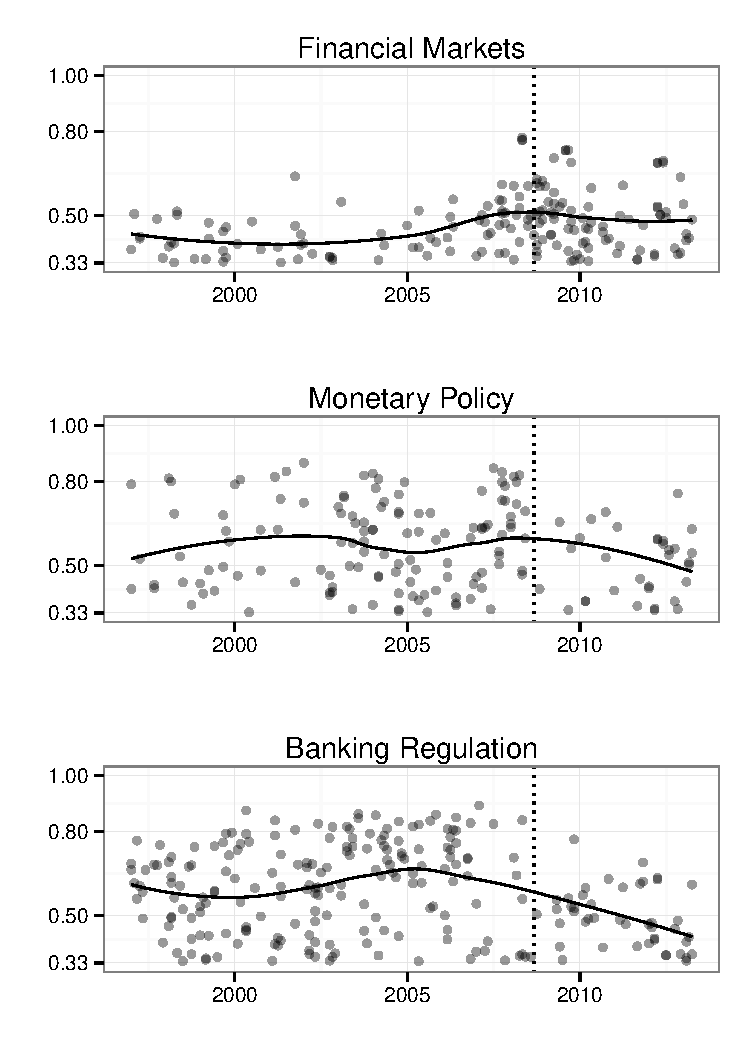
\includegraphics[scale=0.35]{img/TopicBasic.pdf}
    \end{center}

    {\tiny{Source: Young and Gandrud (2016)}}

}

\frame{
    \frametitle{Text analysis in social science (examples)}

    We may have research questions about widely held beliefs across time, for which a survey would be {\large{too costly}} or even impossible to run.

    \vspace{1cm}

    For example, if we wanted to study monthly perceptions of financial market stress across 180 countries.

}

\frame{
    \frametitle{Real-Time Perceptions of Financial Market Stress}


    \begin{center}
        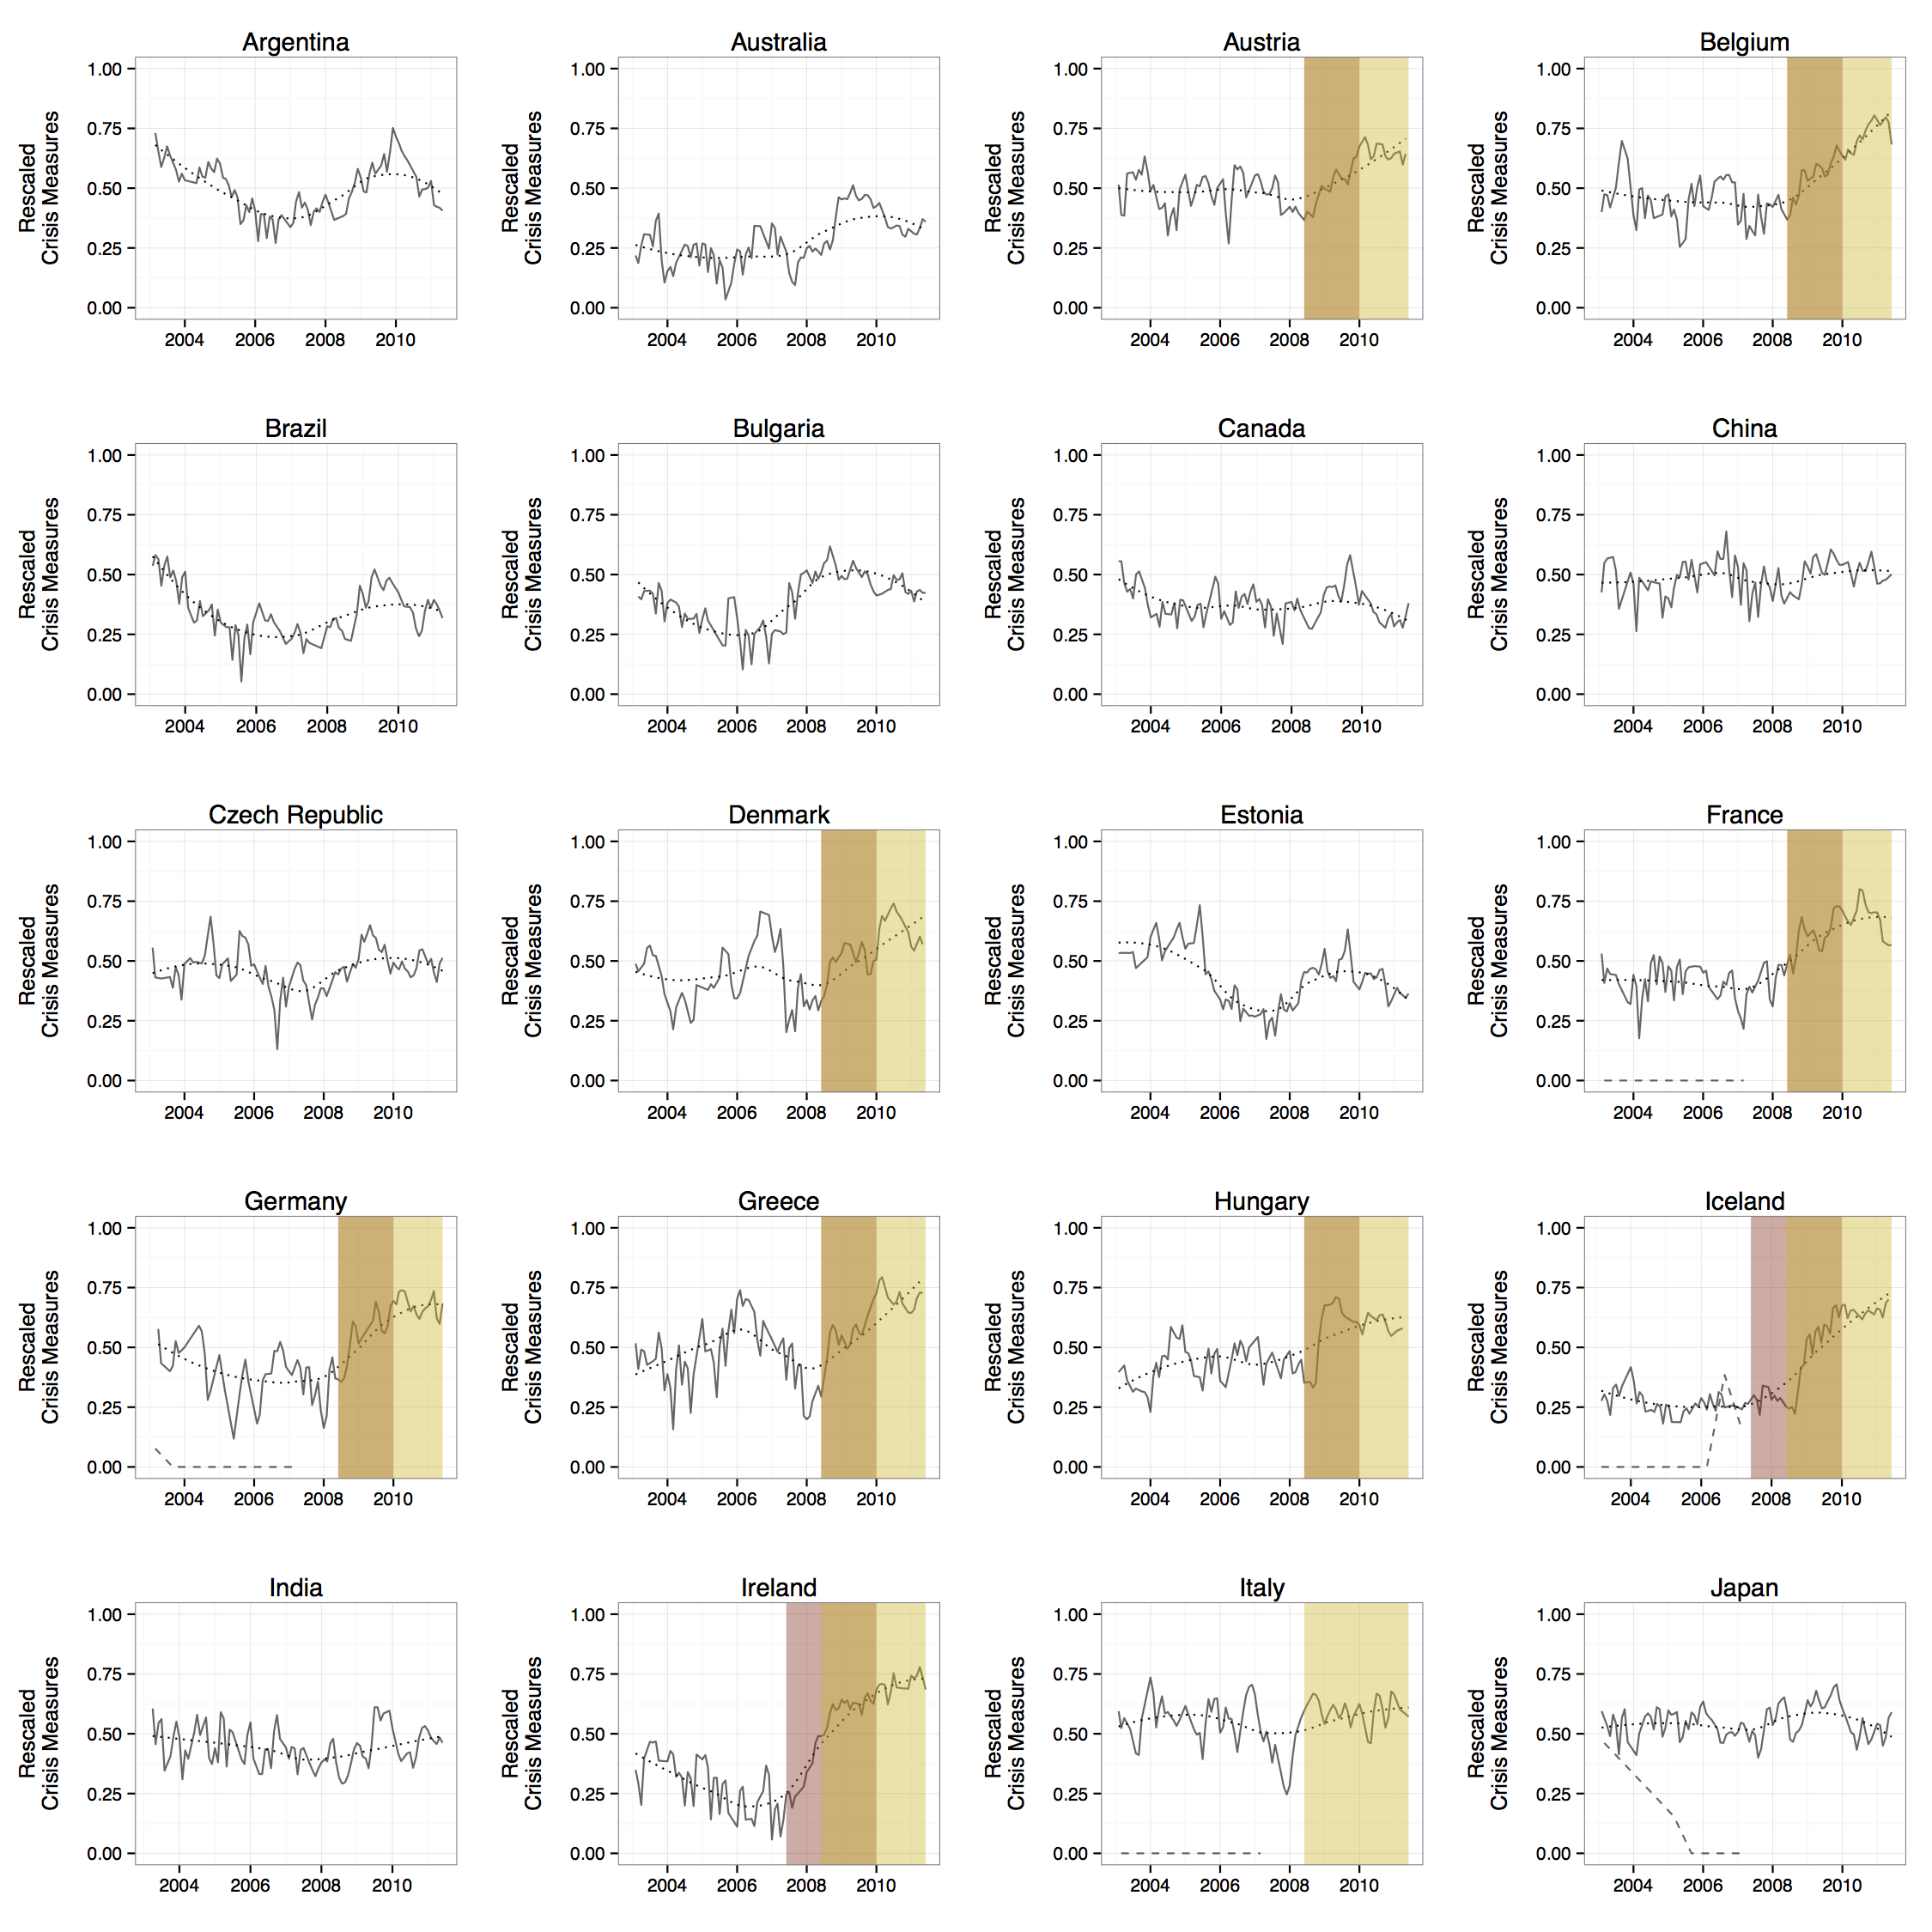
\includegraphics[scale=0.17]{img/perceptions_compare.png}
    \end{center}

    {\tiny{Source: Gandrud and Hallerberg (2016)}}

}

\frame{
    \frametitle{GDELT Global Leaders Press Coverage}

    \begin{center}
        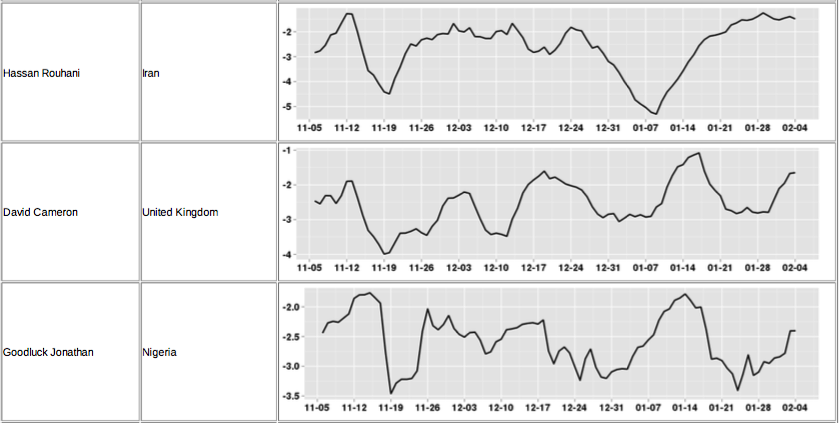
\includegraphics[scale=0.35]{img/gdelt_leaders.png}
    \end{center}

    {\tiny{Source: http://data.gdeltproject.org/worldleadersindex/GDELT\_Leaders\_Index-2016-02-05.pdf}}

}

\frame{
    \frametitle{Common data output}

    Text analysis can create data that is:

    \vspace{0.5cm}

    \begin{itemize}
        \item {\large{Discrete}}: e.g. the main topics of a text.

        \vspace{0.5cm}

        \item {\large{Continuous}}: e.g. proportion of a document dedicated to a specific word or words, scale (negative to positive, left-right).
    \end{itemize}

    \vspace{0.5cm}

    The choice largely depends on your {\large{research question}}.

}


\section{Human and Machine Coding}

\frame{
    \frametitle{Human vs. Machine coding}

    You can analyse texts either by relying exclusively on human coders or also rely on machine-assistance.

}

\frame{
    \frametitle{Human vs. Machine coding}
    Note: you should {\large{never exclusively rely on machine coding}}. At a minimum, you need to check the validity of your machine assigned codes.

    \vspace{0.5cm}

    Do the machine assigned codes make sense in relation to the context?

}

\frame{
    \frametitle{Human vs. Machine coding}

    Machine coding has the advantage of being much more {\large{efficient}} for large numbers of texts.

        \begin{itemize}
            \item For example, it would basically be impossible for GDELT to create a daily updated index of world leader press coverage with human coders.
        \end{itemize}

    \vspace{1cm}

    Machine coding is often more easily {\large{reproducible}} and update-able.
}

\frame{
    \frametitle{Human and Machine coding similarities}

    \begin{center}
        Regardless of whether you use human or machine coding, the general text analysis {\large{process is the same}}.
    \end{center}

}

\section{General Text Analysis Steps}

\frame{
    \frametitle{Text analysis steps}

    \begin{enumerate}

        \item {\large{Define}} the population of texts you are interested in (e.g. press releases by a particular organisation, open-ended survey responses).

        \vspace{0.5cm}

        \item Gather your {\large{sample of texts}}

        \vspace{0.5cm}

        \item {\large{Develop}} a coding scheme and {\large{classify}} your texts.

        \vspace{0.5cm}

        \item Establish the {\large{reliability and validity}} of your classifications.

    \end{enumerate}

    {\tiny{Modified from: http://psc.dss.ucdavis.edu/sommerb/sommerdemo/content/doing.htm}}

}

\frame{
    \frametitle{Population}

    At least two items to consider when defining your population of texts:

    \vspace{0.5cm}

    \begin{itemize}
        \item Should be relevant for your research question.

        \vspace{0.5cm}

        \item Texts should be accessible.
    \end{itemize}

}

\frame{
    \frametitle{Gather your sample}

    As with all data gathering, how you {\large{sample}} your texts can {\large{greatly affect your results}}.

    \vspace{0.5cm}

    For example, if you want to code press attitudes towards immigrants, but only gather articles from \emph{The Guardian}, you will get much different results than if you only sample \emph{The Daily Mail}.

    \vspace{1cm}

    We will discuss sampling in more detail in Week 7.

}

\frame{
    \frametitle{Advanced: web scraping}

    New tools for {\large{automatically gathering--web scraping--}}large numbers of texts from the internet.

    \vspace{1cm}

    Can make the data collection process {\large{dramatically faster}} and {\large{more reproducible}}.

    \vspace{1cm}

    We do not cover these tools in this course.

}

\frame{
    \frametitle{Gather your sample}

    In order to enhance reproducibility, when you gather your sample (your {\large{Corpus}}) it should be {\large{well-organised}} and {\large{electronically available}}.

}

\frame{
    \frametitle{Develop a coding scheme}

    Always consider {\large{reliability}} when developing your coding scheme.

    \begin{itemize}
        \item Will another coder make the same choices given only the information in your coding scheme?
    \end{itemize}

    \vspace{1cm}

    So, always {\large{fully document}} your coding scheme and {\large{explain your rationale}}.

}

\frame{
    \frametitle{Develop a coding scheme (1)}

    Determine if you want to create a {\large{discrete}} (e.g. main topic of the text) or {\large{continuous}} coding scheme (e.g. attitude scale). T

    \vspace{1cm}

    This decision should be based on {\large{relevance to your research question}}.

    \vspace{1cm}

    {\large{Skim}} a sub-sample of the texts to {\large{make a list}} of possible topics or words that would indicate a particular attitude, etc.

}

\frame{
    \frametitle{Develop a coding scheme (2)}

    From this initial list, create {\large{operational definitions}} of your topic categories or scale.

    \begin{itemize}
        \item In order to enable replication, make these definitions as {\large{clear and specific}} as possible.
    \end{itemize}

    \vspace{0.5cm}

    Check that your definitions are {\large{comprehensive}}. Do they cover as many topics, words related to attitudes as possible?

    \vspace{0.5cm}

    Make sure that your definitions are {\large{mutually exclusive}}, i.e. there is {\large{no overlap}}.
}

\frame{

    \begin{center}
        Now, apply your coding scheme.
    \end{center}

}

\frame{
    \frametitle{Check reliability}

    You should always have {\large{at least one other rater}} independently apply your coding scheme.

    \vspace{0.5cm}

    Then check the {\large{level of aggreement}}. Ideally, different coders will give the same codes to the same texts based on the same coding scheme.

        \begin{itemize}
            \item This is known as high {\large{inter-rater reliability}}

            \item Simple tests for this would be a correlation coefficient (for continuous codes) or $X^2$ tests (for discrete codes). Note: a lack of independence between the two raters' scores is what you want.
        \end{itemize}

}

\frame{
    \frametitle{Check reliability}

    If there is considerable disagreement between raters, you need to {\large{re-evaluate your coding scheme}} and possibly {\large{recode your corpus}}.

}

\frame{
    \frametitle{Check machine coded reliability}

    If you used machine coding, then you should {\large{select a random sub-sample}} of the texts and check to see if the machine codes match {\large{your intended coding scheme}}.

}

\section{Special issues with machine coding}

\frame{
    \frametitle{Special issues: machine coding}

    There are many different advanced techniques for machine coding:

    \begin{center}
        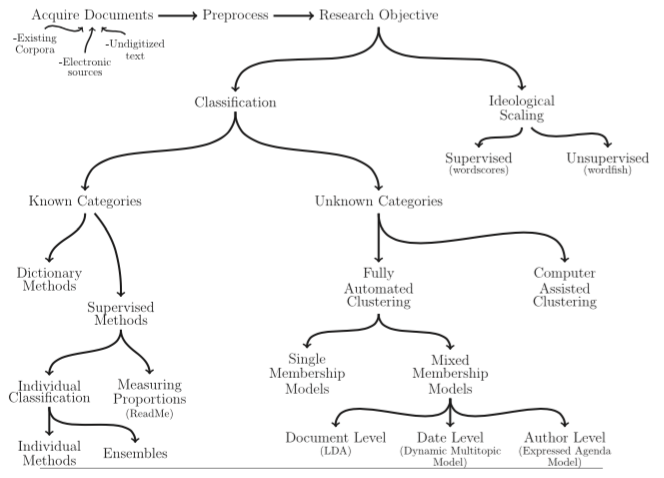
\includegraphics[scale=0.35]{img/grimmer_stewart.png}
    \end{center}

    {\tiny{Grimmer and Stewart (2013, 268)}}

}

\frame{
    \frametitle{This course}

    In this course we will focus on:

    \begin{itemize}
        \item The text {\large{preprocessing step}}.

        \vspace{0.5cm}

        \item {\large{Simple word frequency}} methods of text analysis.
    \end{itemize}

}

\frame{
    \frametitle{Preprecessing}

    Regardless of the type of machine coding you use, you need to {\large{preprocess your texts}}.

    \vspace{1cm}
    This can include\ldots

}

\frame{
    \frametitle{Preprecessing}
        Removing unnecessary white space (spacing between words), punctuation, capitalisation, numbers, etc.
}

\frame{
    \frametitle{Preprecessing}

        Removing {\large{stopwords}}: function words that do not convey meaning like ``a'' and ``the''.

}

\frame{
    \frametitle{Preprecessing}

        {\large{Stem}} your words: reduce the ends of words to reduce the total number of unique words.

        \begin{itemize}

            \item For example: \emph{family}, \emph{\emph{families}}, \emph{families'}, \emph{familial}, are changed to their stem: \emph{famili}.

            \item Stemming is related to linguistic concept called \emph{lemmatization}.

        \end{itemize}

}

\frame{

    \begin{center}
        Note: each preprocessing decision affects your results and so should be {\large{fully justified}}.
    \end{center}
}

\frame{

    \begin{center}
        Once you have preprocessed your data, then you can have your computer code the corpus.
    \end{center}
}

\frame{
    \frametitle{Word frequency}

    In this course, we are going to focus on {\large{word frequency}} methods.

    \vspace{0.5cm}

    Note, you should focus on the {\large{relative requency}} of a word. Most simply:

    \begin{equation}
        \mathrm{Relative\:Frequency} = \frac{\mathrm{Freq.\:of\:word\:in\:text}}{\mathrm{Total\:words\:in\:text}}
    \end{equation}

    \vspace{1cm}

    Corrects for words being more frequent because a text is longer.
}

\frame{
    \frametitle{Word frequency}

        Word frequency is an efficient way to help you {\large{reproducibly summarise}} many texts,

        \begin{center}
            \emph{but\ldots}
        \end{center}

        word frequencies have {\large{have no inherent meaning}}.

        \vspace{0.5cm}

        You still need to code what the frequency of a word means, relative to the context and your research question.

}

\frame{
    \frametitle{Simple example: January 2016 Press Release}

    \begin{center}
        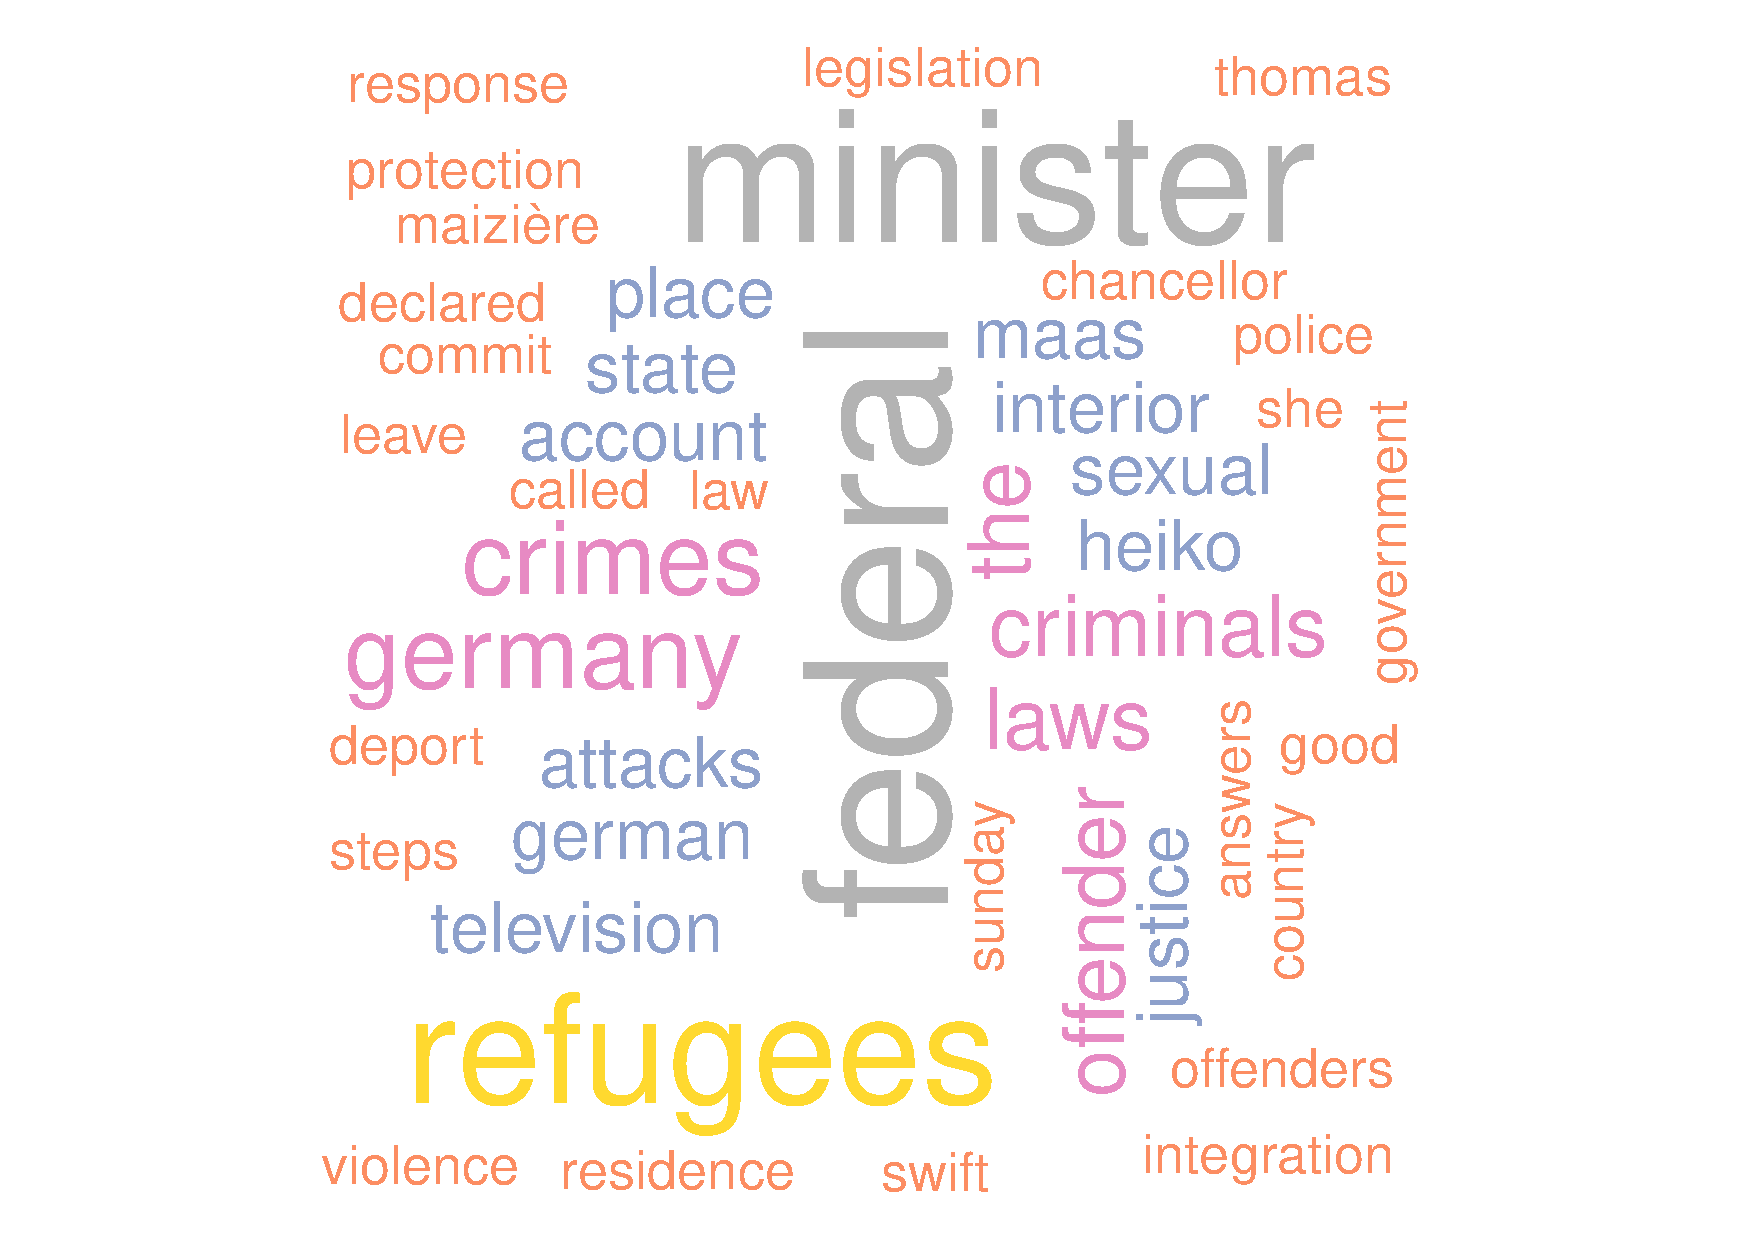
\includegraphics[scale=0.3]{img/jan_chancellor.pdf}
    \end{center}

    Refugees discussed in terms of the topic \ldots

}

\frame{
    \frametitle{Simple example: January 2016 Press Release}

    \begin{center}
        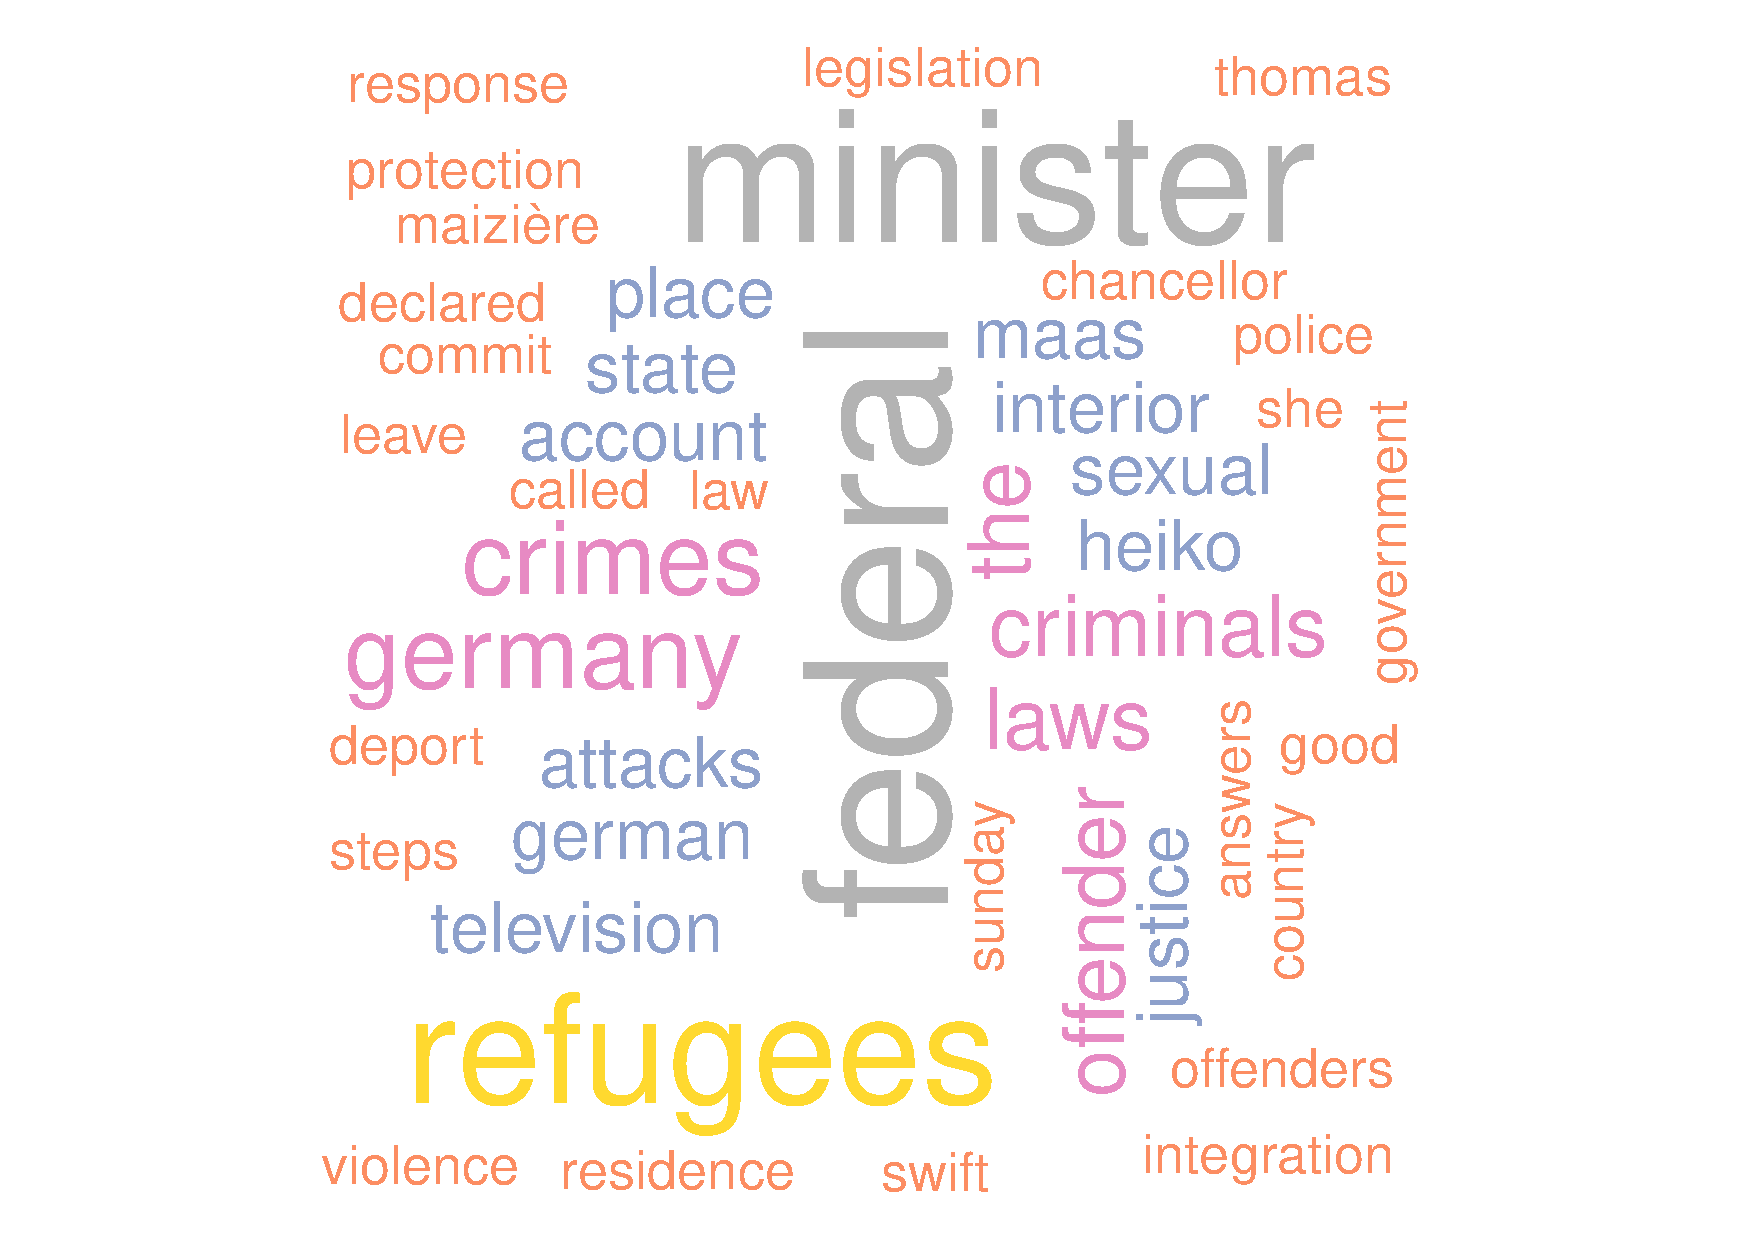
\includegraphics[scale=0.3]{img/jan_chancellor.pdf}
    \end{center}

    Refugees discussed in terms of the topic \emph{crimminality}.

}

\section{Pros and Cons}

\frame{
    \frametitle{Some Pros and Cons of Text Analysis}

    \begin{table}
        {\footnotesize{
        \begin{tabular}{p{4.5cm} p{4.5cm}}
            {\large{Pros}} & {\large{Cons}} \\
            \hline\hline \\[0.1cm]
            Texts are a massive new source of social data & Results can be misleading if we don't appreciate the context within which the speech acts takes place. \\[0.3cm]
            Useful for tracking changes over time & Purely descriptive, need to do more work to understand why \\[0.3cm]
            Can be an inexpensive way to gather social data & Sampling bias (including if writers delete texts) can be a major challenge \\[0.1cm]
            \hline
        \end{tabular}
        }}
    \end{table}

    {\tiny{Partially from http://psc.dss.ucdavis.edu/sommerb/sommerdemo/content/strengths.htm}}

}


\end{document}
